% Options for packages loaded elsewhere
\PassOptionsToPackage{unicode}{hyperref}
\PassOptionsToPackage{hyphens}{url}
%
\documentclass[
]{article}
\usepackage{lmodern}
\usepackage{amsmath}
\usepackage{ifxetex,ifluatex}
\ifnum 0\ifxetex 1\fi\ifluatex 1\fi=0 % if pdftex
  \usepackage[T1]{fontenc}
  \usepackage[utf8]{inputenc}
  \usepackage{textcomp} % provide euro and other symbols
  \usepackage{amssymb}
\else % if luatex or xetex
  \usepackage{unicode-math}
  \defaultfontfeatures{Scale=MatchLowercase}
  \defaultfontfeatures[\rmfamily]{Ligatures=TeX,Scale=1}
\fi
% Use upquote if available, for straight quotes in verbatim environments
\IfFileExists{upquote.sty}{\usepackage{upquote}}{}
\IfFileExists{microtype.sty}{% use microtype if available
  \usepackage[]{microtype}
  \UseMicrotypeSet[protrusion]{basicmath} % disable protrusion for tt fonts
}{}
\makeatletter
\@ifundefined{KOMAClassName}{% if non-KOMA class
  \IfFileExists{parskip.sty}{%
    \usepackage{parskip}
  }{% else
    \setlength{\parindent}{0pt}
    \setlength{\parskip}{6pt plus 2pt minus 1pt}}
}{% if KOMA class
  \KOMAoptions{parskip=half}}
\makeatother
\usepackage{xcolor}
\IfFileExists{xurl.sty}{\usepackage{xurl}}{} % add URL line breaks if available
\IfFileExists{bookmark.sty}{\usepackage{bookmark}}{\usepackage{hyperref}}
\hypersetup{
  pdftitle={Supplement to Smith et al.: Assessing the effect of article processing charges on the geographic diversity of authors using Elsevier's `Mirror Journal' system},
  pdfauthor={A. C. Smith, L. Merz, J. B. Borden, C. K. Gulick, A. R. Kshirsagar, and E. M. Bruna},
  hidelinks,
  pdfcreator={LaTeX via pandoc}}
\urlstyle{same} % disable monospaced font for URLs
\usepackage[margin=1in]{geometry}
\usepackage{graphicx}
\makeatletter
\def\maxwidth{\ifdim\Gin@nat@width>\linewidth\linewidth\else\Gin@nat@width\fi}
\def\maxheight{\ifdim\Gin@nat@height>\textheight\textheight\else\Gin@nat@height\fi}
\makeatother
% Scale images if necessary, so that they will not overflow the page
% margins by default, and it is still possible to overwrite the defaults
% using explicit options in \includegraphics[width, height, ...]{}
\setkeys{Gin}{width=\maxwidth,height=\maxheight,keepaspectratio}
% Set default figure placement to htbp
\makeatletter
\def\fps@figure{htbp}
\makeatother
\setlength{\emergencystretch}{3em} % prevent overfull lines
\providecommand{\tightlist}{%
  \setlength{\itemsep}{0pt}\setlength{\parskip}{0pt}}
\setcounter{secnumdepth}{-\maxdimen} % remove section numbering
\usepackage{fancyhdr}
\pagestyle{fancy}
\fancyfoot{}
\fancyhead[L]{APCs and Author Diversity (Supplement)}
\fancyhead[R]{p. \thepage}
\usepackage{setspace}
\usepackage{parskip}
\usepackage{pdflscape}
\newcommand{\blandscape}{\begin{landscape}}
\newcommand{\elandscape}{\end{landscape}}
\usepackage{caption}
\DeclareCaptionLabelFormat{Sformat}{#1 S#2}
\captionsetup[table]{labelformat=Sformat}
\captionsetup[figure]{labelformat=Sformat}
\usepackage{booktabs}
\usepackage{longtable}
\usepackage{array}
\usepackage{multirow}
\usepackage{wrapfig}
\usepackage{float}
\usepackage{colortbl}
\usepackage{pdflscape}
\usepackage{tabu}
\usepackage{threeparttable}
\usepackage{threeparttablex}
\usepackage[normalem]{ulem}
\usepackage{makecell}
\usepackage{xcolor}
\ifluatex
  \usepackage{selnolig}  % disable illegal ligatures
\fi

\title{Supplement to Smith et al.: Assessing the effect of article
processing charges on the geographic diversity of authors using
Elsevier's `Mirror Journal' system}
\author{A. C. Smith, L. Merz, J. B. Borden, C. K. Gulick, A. R.
Kshirsagar, and E. M. Bruna}
\date{}

\begin{document}
\maketitle

\newpage
\begin{figure}

{\centering 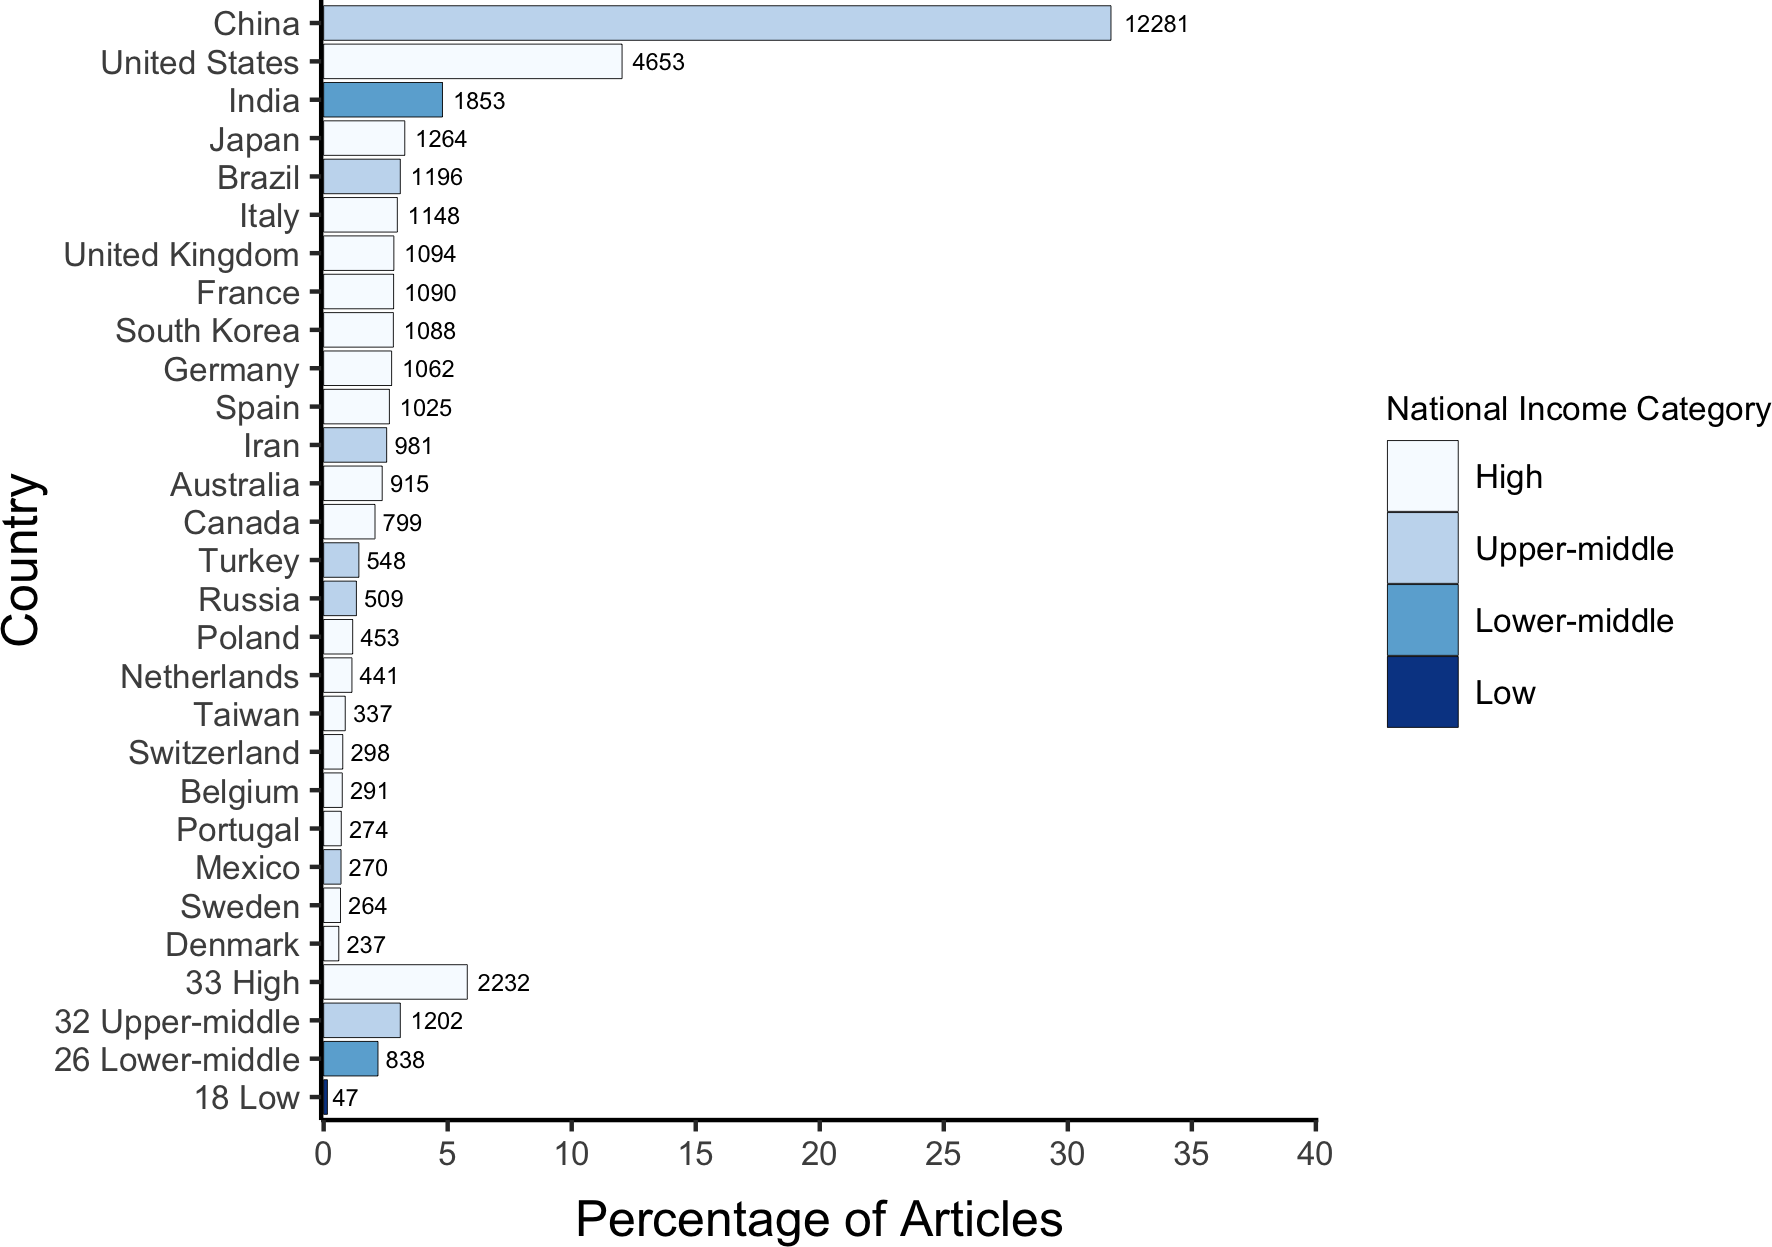
\includegraphics{Smith_etal_QSS_Supplement_files/figure-latex/FigS1-1} 

}

\caption{Percentage of lead authors (i..e, first and single-authors) based in different countries; Parent and Mirror journals combined. Numbers adjacent to bars are the number of articles with lead authors based in that country.}\label{fig:FigS1}
\end{figure}

\newpage
\blandscape

\begin{figure}

{\centering 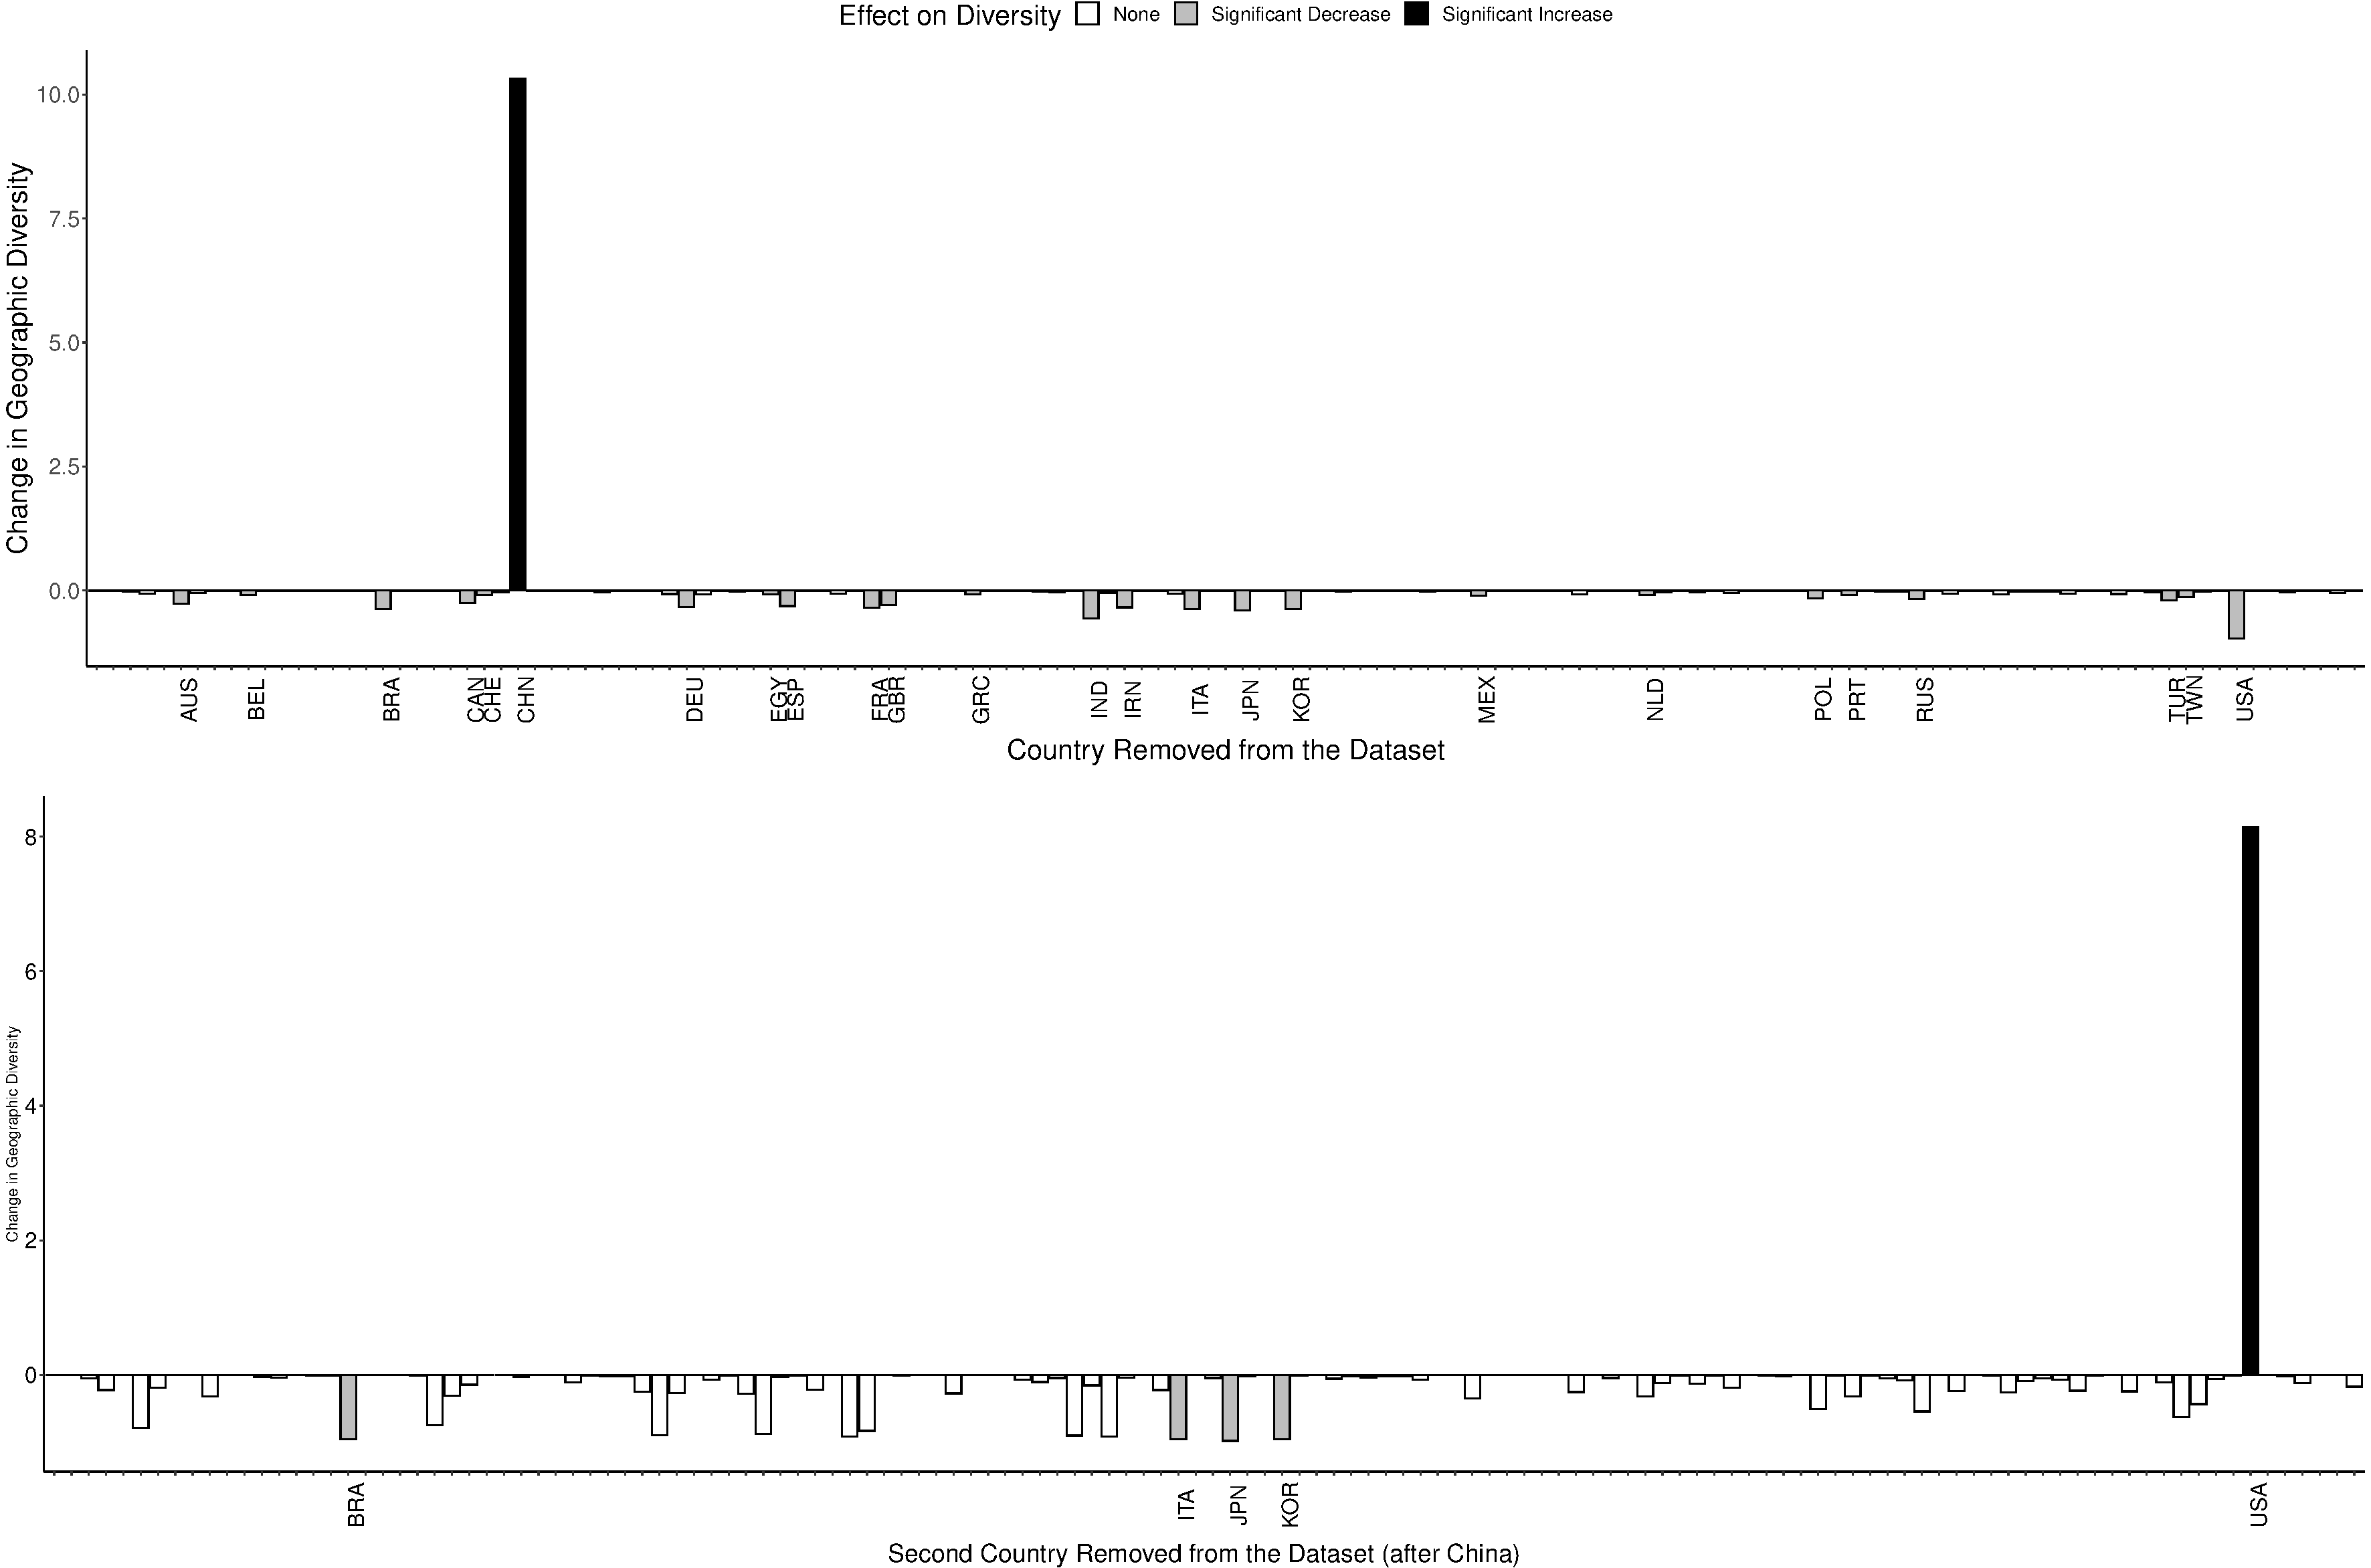
\includegraphics{Smith_etal_QSS_Supplement_files/figure-latex/FigS2-1} 

}

\caption{The effect on $D_{2}$ of excluding authors from individual countries (B) The effect on $D_{2}$ of excluding authors from individual countries after having first removed China.}\label{fig:FigS2}
\end{figure}

\elandscape
\newpage

\begin{figure}

{\centering 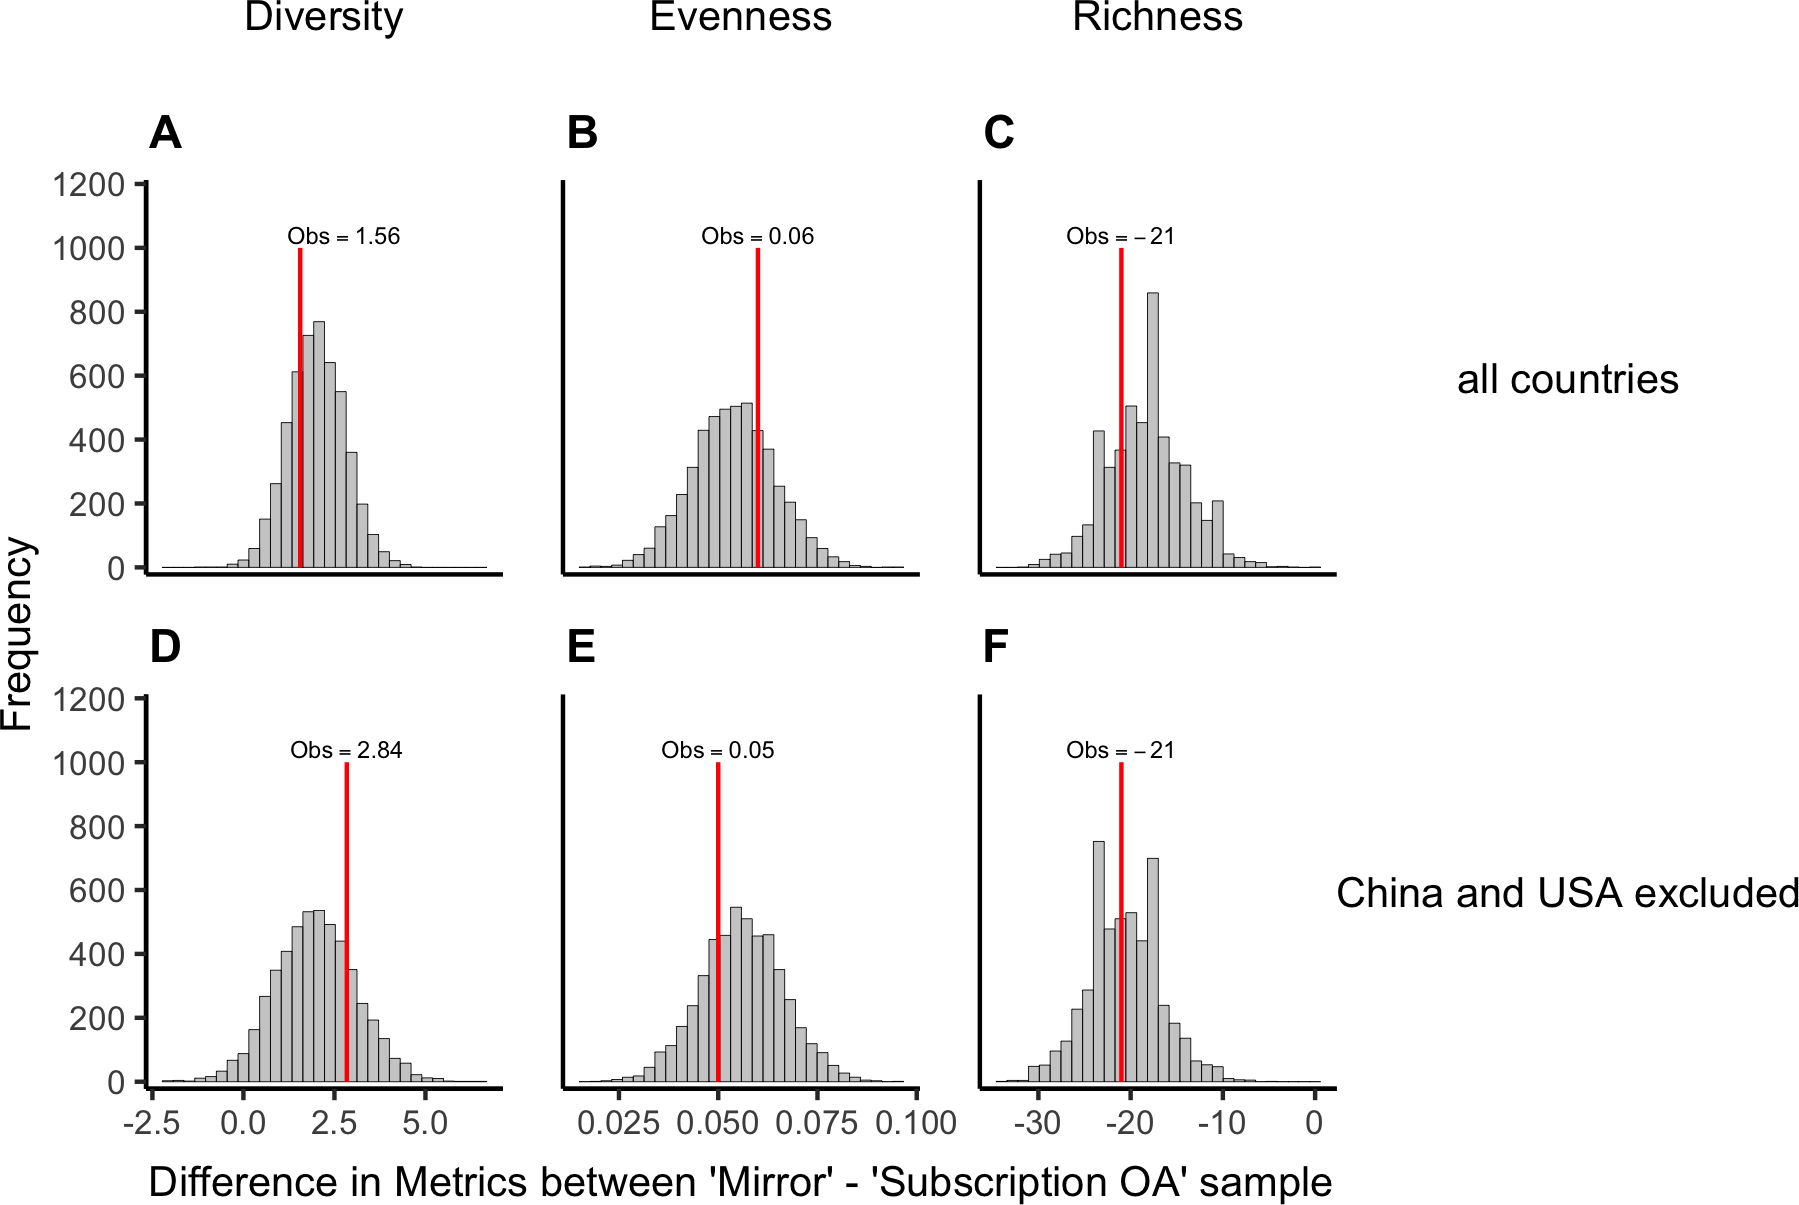
\includegraphics{Smith_etal_QSS_Supplement_files/figure-latex/FigS3-1} 

}

\caption{Results of permutation tests comparing author Diversity, Richness, and Evenness of open access articles published in Parent and Mirror journals. The line indicates the observed difference between the two populations, while the bars represent the frequency in 5000 permutations of the difference between two groups identical in size and structure to the observed collections but to which articles were assigned at random without replacement. Results are shown for analyses including all countries (A-C) and when excluding articles by first- and single-authors based in China or the USA (D-F). Note also that these analyses were conducted by pooling first- and single-author articles within each journal type; we were unable to do permutation tests comparing by authorship category (e.g., single-author in Mirror vs. Parent, first-author in Mirror vs. Parent) because several journals had no articles in one of the categories; alternative attempts to test for differences using bootstrapping did not suggest there were significant differences in diversity when comparing by category.}\label{fig:FigS3}
\end{figure}

\begin{figure}

{\centering 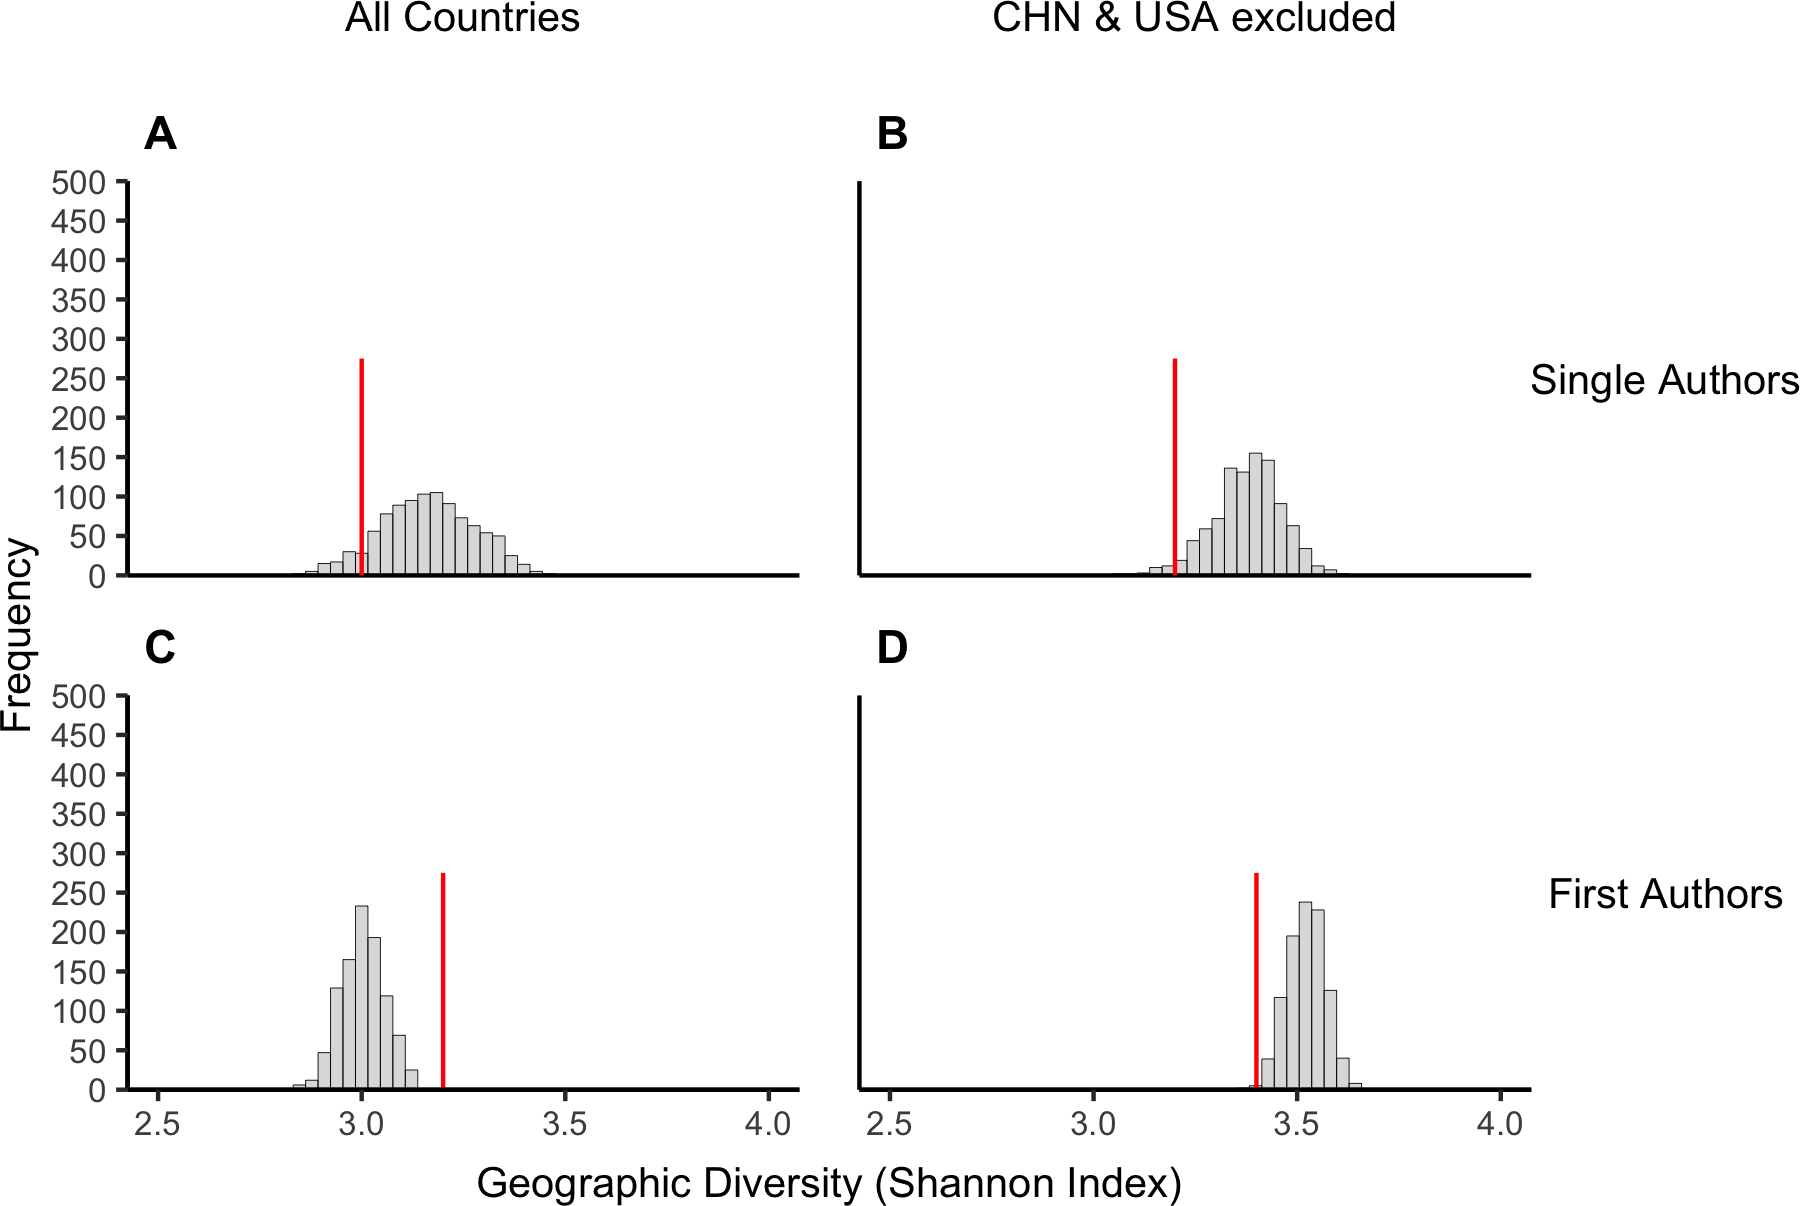
\includegraphics{Smith_etal_QSS_Supplement_files/figure-latex/FigS4-1} 

}

\caption{Author Geographic Diversity (Shannon's Index) for N =  975  articles in Mirror journals (solid line) and 1000 identically sized collections generated by selecting an identical number of non-open access articles in Parent journals by bootstrapping from the pool of N =  34400  total articles. Results are shown for analyses including all countries (A, C) and when excluding artciles by first- and single-authors based in China or the USA (B, D).}\label{fig:FigS4}
\end{figure}

\begin{figure}

{\centering 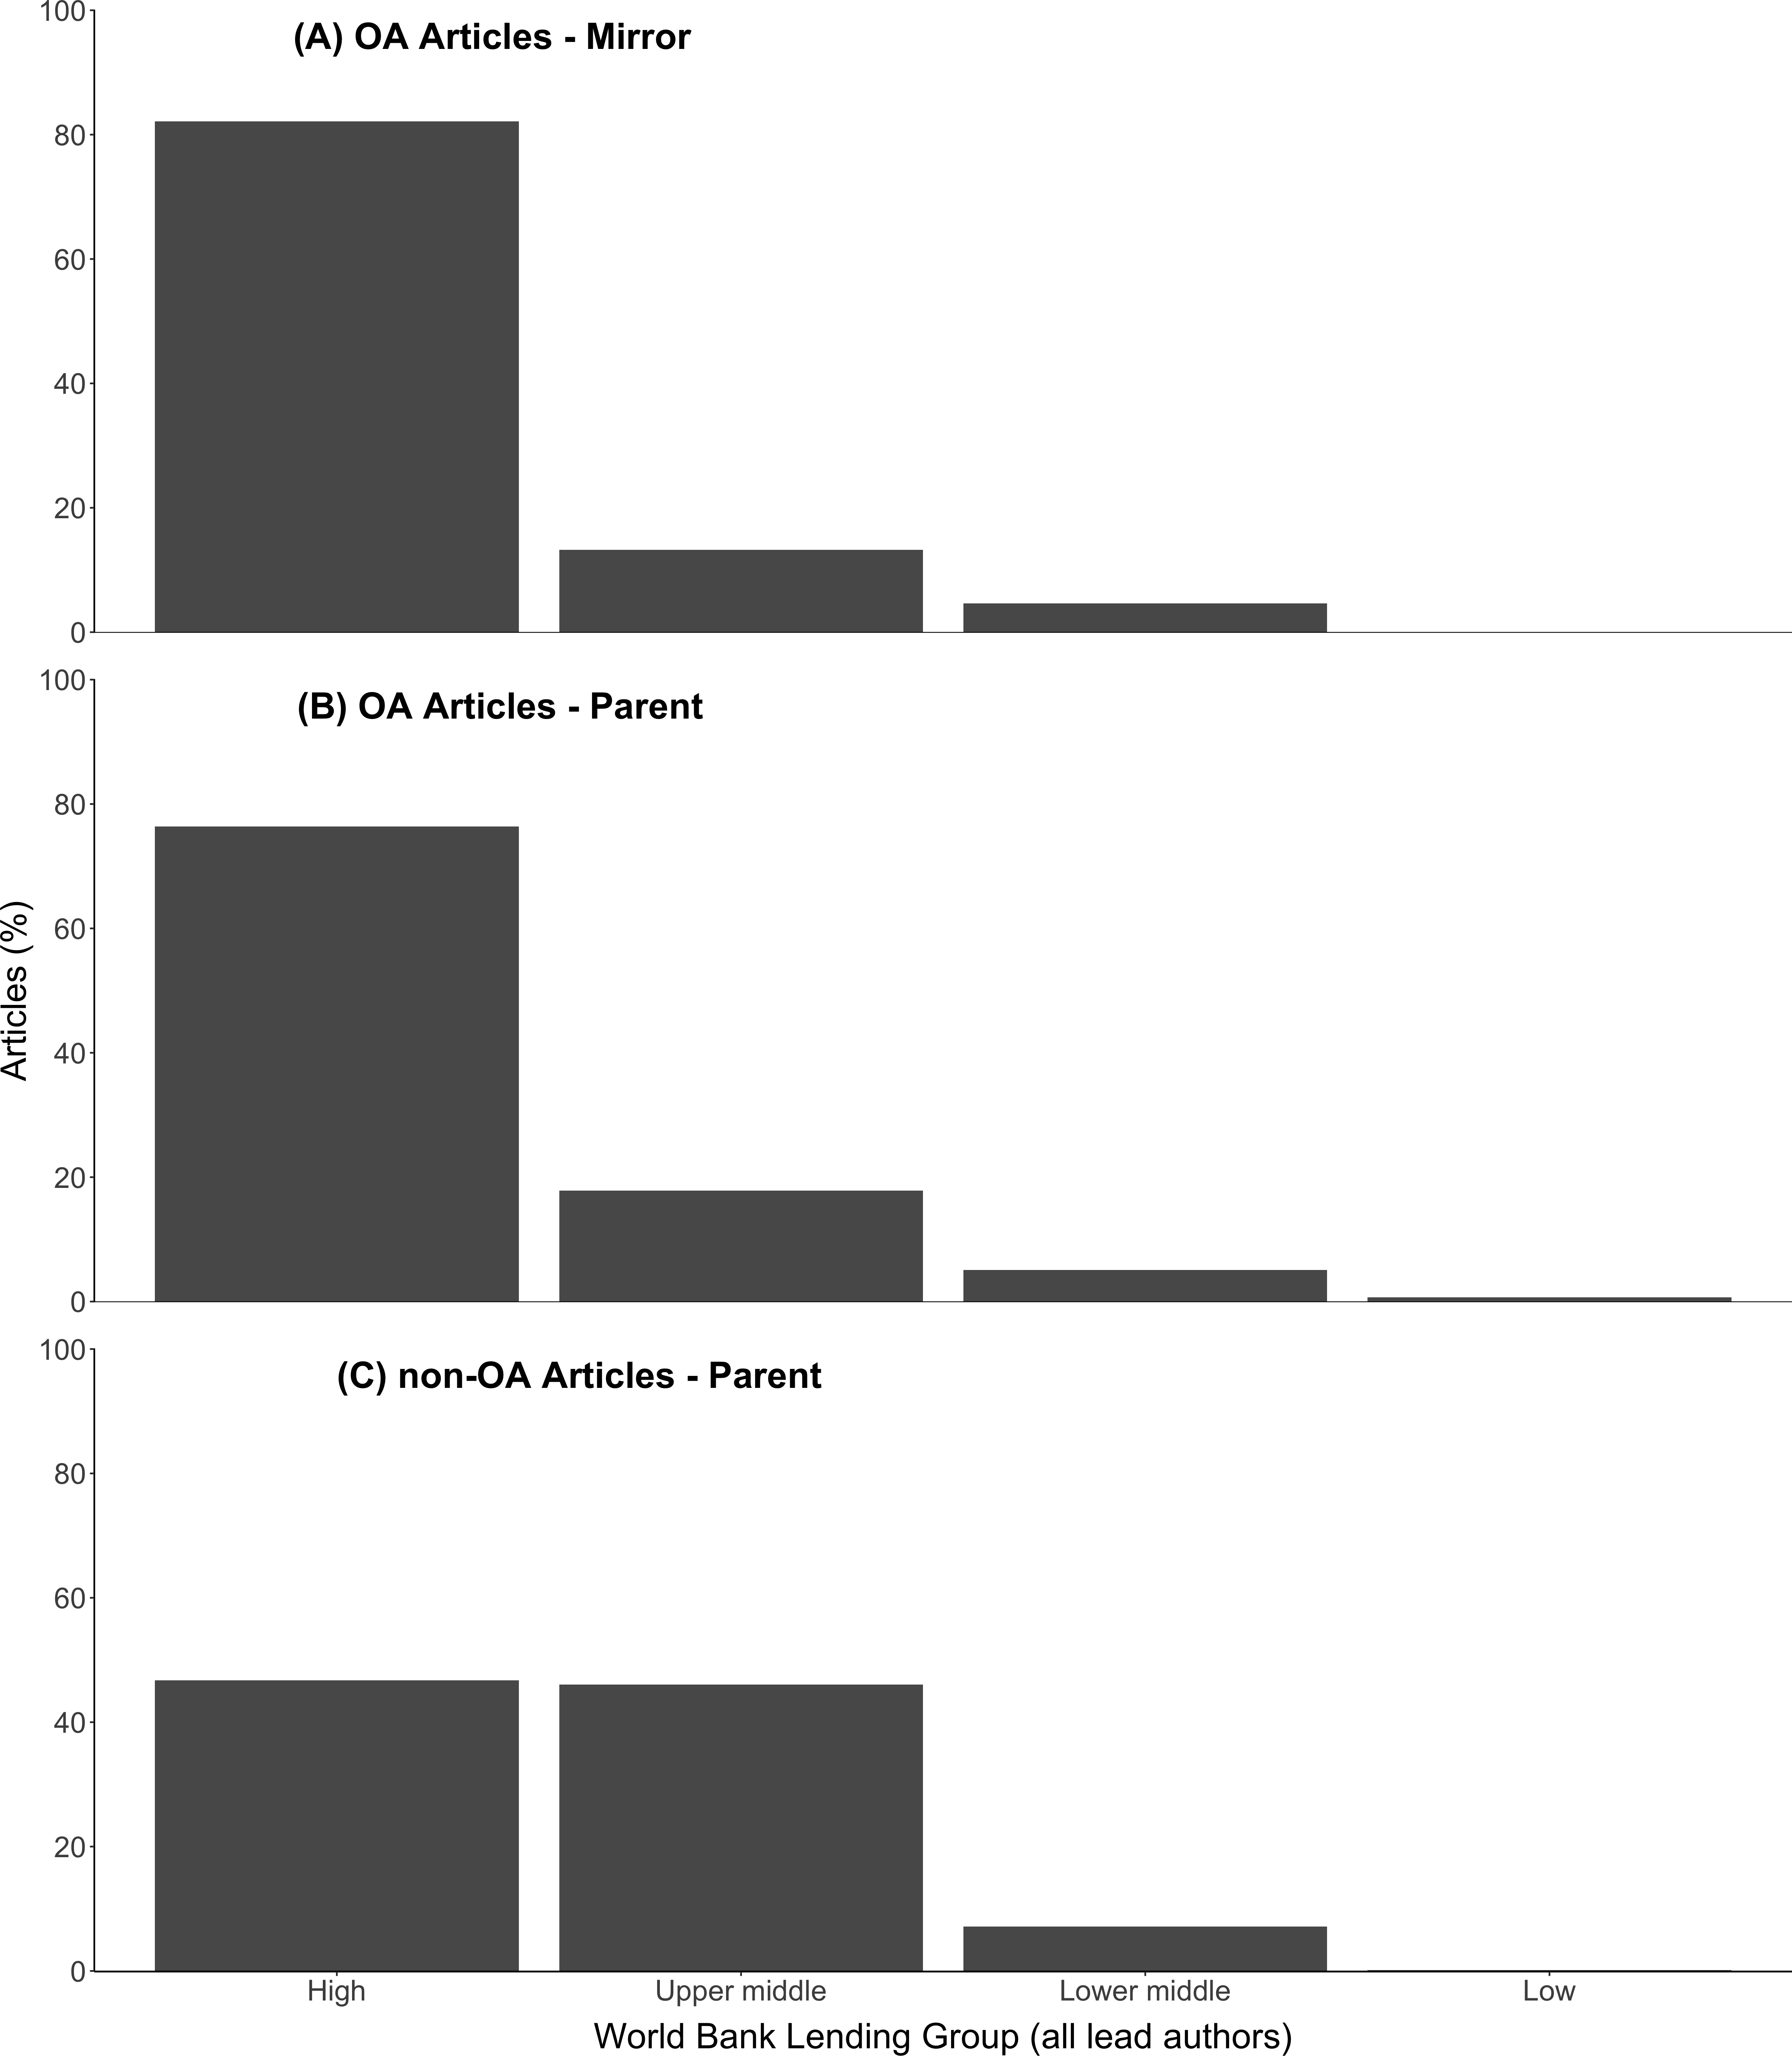
\includegraphics{Smith_etal_QSS_Supplement_files/figure-latex/FigS5-1} 

}

\caption{Proportion of lead authors based in different World Bank Lending Groups when pooling all of the (A) N =  975  articles in open access (OA) Mirror journals, (B) N =   1832  OA articles in Parent journals, and (C) N =   34400  non-OA articles in Parent journals.}\label{fig:FigS5}
\end{figure}

\newpage
\blandscape

\begin{table}

\caption{\label{tab:TableS1}Countries eligible for APC waivers through Elsevier's 'Research4Life' program by World Bank Global Region and Income Group.}
\resizebox{\linewidth}{!}{
\fontsize{12}{14}\selectfont
\begin{tabular}[t]{ccccc}
\toprule
Region & Income Group & A - 100\% & B - 50\% & no waiver\\
\midrule
South Asia & Low income & Afghanistan, Nepal & - & -\\
 & Middle income & Bangladesh, Bhutan & Maldives, Pakistan, Sri Lanka & India\\
\cline{1-5}
Sub-Saharan Africa & Low income & Benin, Burkina Faso, Burundi & - & -\\
 &  & Central African Republic, Chad, Dem. Repub. Congo, Eritrea & - & -\\
 &  & Ethiopia, Gambia, Guinea, Guinea-Bissau & - & -\\
 &  & Liberia, Madagascar, Malawi, Mali & - & -\\
 &  & Mozambique, Niger, Rwanda, Sierra Leone & - & -\\
 &  & Somalia, South Sudan, Tanzania, Togo & - & -\\
 &  & Uganda & - & -\\
 & Middle income & Angola, Cabo Verde, Cameroon & Botswana, Gabon, Mauritius & South Africa\\
 &  & Comoros, Congo, Equatorial Guinea, Eswatini & Namibia, Nigeria & -\\
 &  & Ghana, Ivory Coast, Kenya, Lesotho & - & -\\
 &  & Mauritania, Sao Tome \& Principe, Senegal, Sudan & - & -\\
 &  & Zambia, Zimbabwe & - & -\\
 & High income & - & Seychelles & -\\
\cline{1-5}
Latin America \& Caribbean & Low income & Haiti & - & -\\
 & Middle income & Belize, Nicaragua & Bolivia, Colombia, Cuba & Argentina, Brazil, Costa Rica\\
 &  & - & Dominica, Ecuador, El Salvador, Grenada & Dominican Republic, Mexico\\
 &  & - & Guatemala, Guyana, Honduras, Jamaica & -\\
 &  & - & Paraguay, Peru, Saint Lucia, Saint Vincent \& the Grenadines & -\\
 &  & - & Suriname, Venezuela & -\\
 & High income & - & Antigua \& Barbuda, Saint Kitts \& Nevis & Aruba, Bahamas, Barbados\\
 &  & - & - & British Virgin Islands, Cayman Islands, Chile, Curaçao\\
 &  & - & - & Panama, Puerto Rico, Saint Martin (FRA), Sint Maarten\\
 &  & - & - & Trinidad \& Tobago, Turks \& Caicos Islands, U.S. Virgin Islands, Uruguay\\
\cline{1-5}
Middle East \& North Africa & Low income & Syrian Arab Republic, Yemen & - & -\\
 & Middle income & Djibouti & Algeria, Egypt, Iraq & Iran, Lebanon\\
 &  & - & Jordan, Libya, Morocco, Tunisia & -\\
 &  & - & West Bank \& Gaza Strip & -\\
 & High income & - & - & Bahrain, Israel, Kuwait\\
 &  & - & - & Malta, Oman, Qatar, Saudi Arabia\\
 &  & - & - & United Arab Emirates\\
\cline{1-5}
E. Asia \& Pacific & Low income & Democratic People’s Republic  Korea & - & -\\
 & Middle income & Cambodia, Fed. States  Micronesia, Kiribati & Fiji, Mongolia, Nauru & American Samoa, China, Indonesia\\
 &  & Laos, Marshall Islands, Myanmar, Papua New Guinea & Vietnam & Malaysia, Philippines, Thailand\\
 &  & Samoa, Solomon Islands, Timor-Leste, Tonga & - & -\\
 &  & Tuvalu, Vanuatu & - & -\\
 & High income & - & Palau & Australia, Brunei, French Polynesia\\
 &  & - & - & Guam, Hong Kong, Japan, Macao\\
 &  & - & - & N. Mariana Islands, New Caledonia, New Zealand, Singapore\\
 &  & - & - & South Korea, Taiwan\\
 &  & Tokelau & Cook Islands, Niue & -\\
\cline{1-5}
Europe \& Central Asia & Low income & Tajikistan & - & -\\
 & Middle income & Kyrgyzstan, Republic  Moldova & Albania, Armenia, Azerbaijan & Bulgaria, Kazakhstan, Romania\\
 &  & - & Belarus, Bosnia \& Herzegovina, Georgia, Kosovo & Russia, Turkey, Turkmenistan\\
 &  & - & Montenegro, North Macedonia, Serbia, Ukraine & -\\
 &  & - & Uzbekistan & -\\
 & High income & - & - & Andorra, Austria, Belgium\\
 &  & - & - & Croatia, Cyprus, Czechia, Denmark\\
 &  & - & - & Estonia, Faroe Islands, Finland, France\\
 &  & - & - & Germany, Gibraltar, Greece, Greenland\\
 &  & - & - & Hungary, Iceland, Ireland, Isle  Man\\
 &  & - & - & Italy, Latvia, Liechtenstein, Lithuania\\
 &  & - & - & -\\
 &  & - & Saint Helena & -\\
\cline{1-5}
North America & High income & - & - & Bermuda, Canada, United States\\
\bottomrule
\end{tabular}}
\end{table}

\end{landscape}
\newpage
\begin{table}[!h]

\caption{\label{tab:TableS2}Results of permutation tests comparing the difference in diversity and richness of (A) articles in Mirror journals and (B) open access articles in parent journals.}
\centering
\resizebox{\linewidth}{!}{
\fontsize{12}{14}\selectfont
\begin{tabular}[t]{llcccc}
\toprule
Countries & Metric & Mirror (OA) & Parent (OA) & Obs. Diff. & $\hat{P}$\\
\midrule
All Countries & Diversity & 14.83 & 13.27 & 1.56 & 27.98\\
 & Richness & 64.00 & 85.00 & -21.00 & 21.82\\
 & Evenness & 0.77 & 0.72 & 0.06 & 72.34\\
NA & NA & NA & NA & NA & NA\\
China and USA excluded & Diversity & 20.08 & 17.24 & 2.84 & 78.54\\
 & Richness & 62.00 & 83.00 & -21.00 & 41.52\\
 & Evenness & 0.82 & 0.76 & 0.05 & 28.18\\
\bottomrule
\end{tabular}}
\end{table}
\pagebreak
\newpage
\begin{table}[!h]

\caption{\label{tab:TableS3}Geographic Evenness and Richness of lead authors publishing Open Access (i.e., OA) articles in Mirror and Parent journals vs. subscription-only, non-OA, articles in Parent journals (Psub). The value for Psub is the mean of 1000 bootstrap-generated article collections identical in size and structure to each OA group with which they are being compared (i.e., OA in Mirror, OA in Parent). Single: authors of single-authored articles; First: first authors of co-authored articles.}
\centering
\resizebox{\linewidth}{!}{
\fontsize{12}{14}\selectfont
\begin{tabular}[t]{lllrccrcc}
\toprule
\multicolumn{3}{c}{ } & \multicolumn{3}{c}{All Countries} & \multicolumn{3}{c}{China \& USA Excluded} \\
\cmidrule(l{3pt}r{3pt}){4-6} \cmidrule(l{3pt}r{3pt}){7-9}
Metric & OA Source & Author & OA & Psub (mean ± SD) & $\hat{P}$ & OA & Psub (mean ± SD) & $\hat{P}$\\
\midrule
Evenness & Mirror & First & 0.78 & 0.73 ± 0.01 & 0.00 & 0.82 & 0.85 ± 0.01 & 0.00\\
 &  & Single & 0.82 & 0.84 ± 0.03 & 0.00 & 0.88 & 0.92 ± 0.02 & 0.00\\
 & Parent & First & 0.71 & 0.74 ± 0.01 & 0.00 & 0.76 & 0.83 ± 0.01 & 0.00\\
 &  & Single & 0.88 & 0.91 ± 0.07 & 0.00 & 0.94 & 0.92 ± 0.1 & 0.19\\
 &  & NA & NA & NA & NA & NA & NA & NA\\
Richness & Mirror & First & 63 & 60.94 ± 3.25 & 0.69 & 61 & 62.58 ± 3.37 & 0.49\\
 &  & Single & 38 & 43.08 ± 2.71 & 0.02 & 36 & 40.01 ± 2.59 & 0.16\\
 & Parent & First & 85 & 70.38 ± 3.17 & 1.00 & 83 & 70 ± 3.17 & 1.00\\
 &  & Single & 15 & 15.52 ± 1.83 & 0.30 & 14 & 13.29 ± 1.47 & 0.79\\
\bottomrule
\end{tabular}}
\end{table}

\newpage
\begin{table}

\caption{\label{tab:TableS4}Number of Open Access (OA) and non-OA articles in Mirror and Parent journals. Values are given for both the collection of articles with all countries included and the one from which first authors based in China or the USA are excluded.}
\centering
\resizebox{\linewidth}{!}{
\fontsize{12}{14}\selectfont
\begin{tabular}[t]{llcc}
\toprule
\multicolumn{2}{c}{ } & \multicolumn{2}{c}{Number of Articles} \\
\cmidrule(l{3pt}r{3pt}){3-4}
Author & Category & All Countries & China and USA Excluded\\
\midrule
Coauthored & OA - Mirror & 768 & 571\\
 & OA in Parent & 1804 & 1271\\
 & non-OA in Parent & 33644 & 18112\\
Single Author & OA - Mirror & 207 & 142\\
 & OA in Parent & 28 & 20\\
 & non-OA in Parent & 756 & 560\\
\midrule
 &  & 37207 & 20676\\
\bottomrule
\end{tabular}}
\end{table}

\end{document}
